\section{Introduction}
\label{sec:intro}

Post-training turns a pretrained language model into a model with a different
behavioral profile.  The same architecture and tokenizer can become a general
instruction follower, a math specialist, or a student distilled from a
reasoning-RL teacher \citep{deepseek-r1-2025}.  These variants are usually
compared at the output: answer accuracy, likelihood, or benchmark score.

Output comparison leaves an internal question open.  Two models may solve the
same problem correctly via different computational paths: a short algebraic
derivation or a longer trace with intermediate checks.  If these behaviors
leave different hidden-state
trajectories, the difference should be measurable before selecting a final
answer or applying an intervention.

We treat measurement and use as separate hypotheses.  For each generated
token, we record the last-position hidden state at every layer.  At one layer,
the resulting sequence is a path through a high-dimensional residual space.  We
summarize that path with a \emph{geometric signature}: a matrix indexed by
trajectory metric and layer.  Each cell is an area under the receiver operating
characteristic curve (AUC) for separating incorrect from correct generations
after log-length residualization.  Values near $0.5$ carry little correctness information;
values farther from $0.5$ indicate a signed association.  We then test the same
trajectory signal at three increasingly demanding evidence levels:
observability, candidate selection, and intervention.  Figure~\ref{fig:overview}
shows the complete protocol.

\begin{figure*}[tbp]
\centering
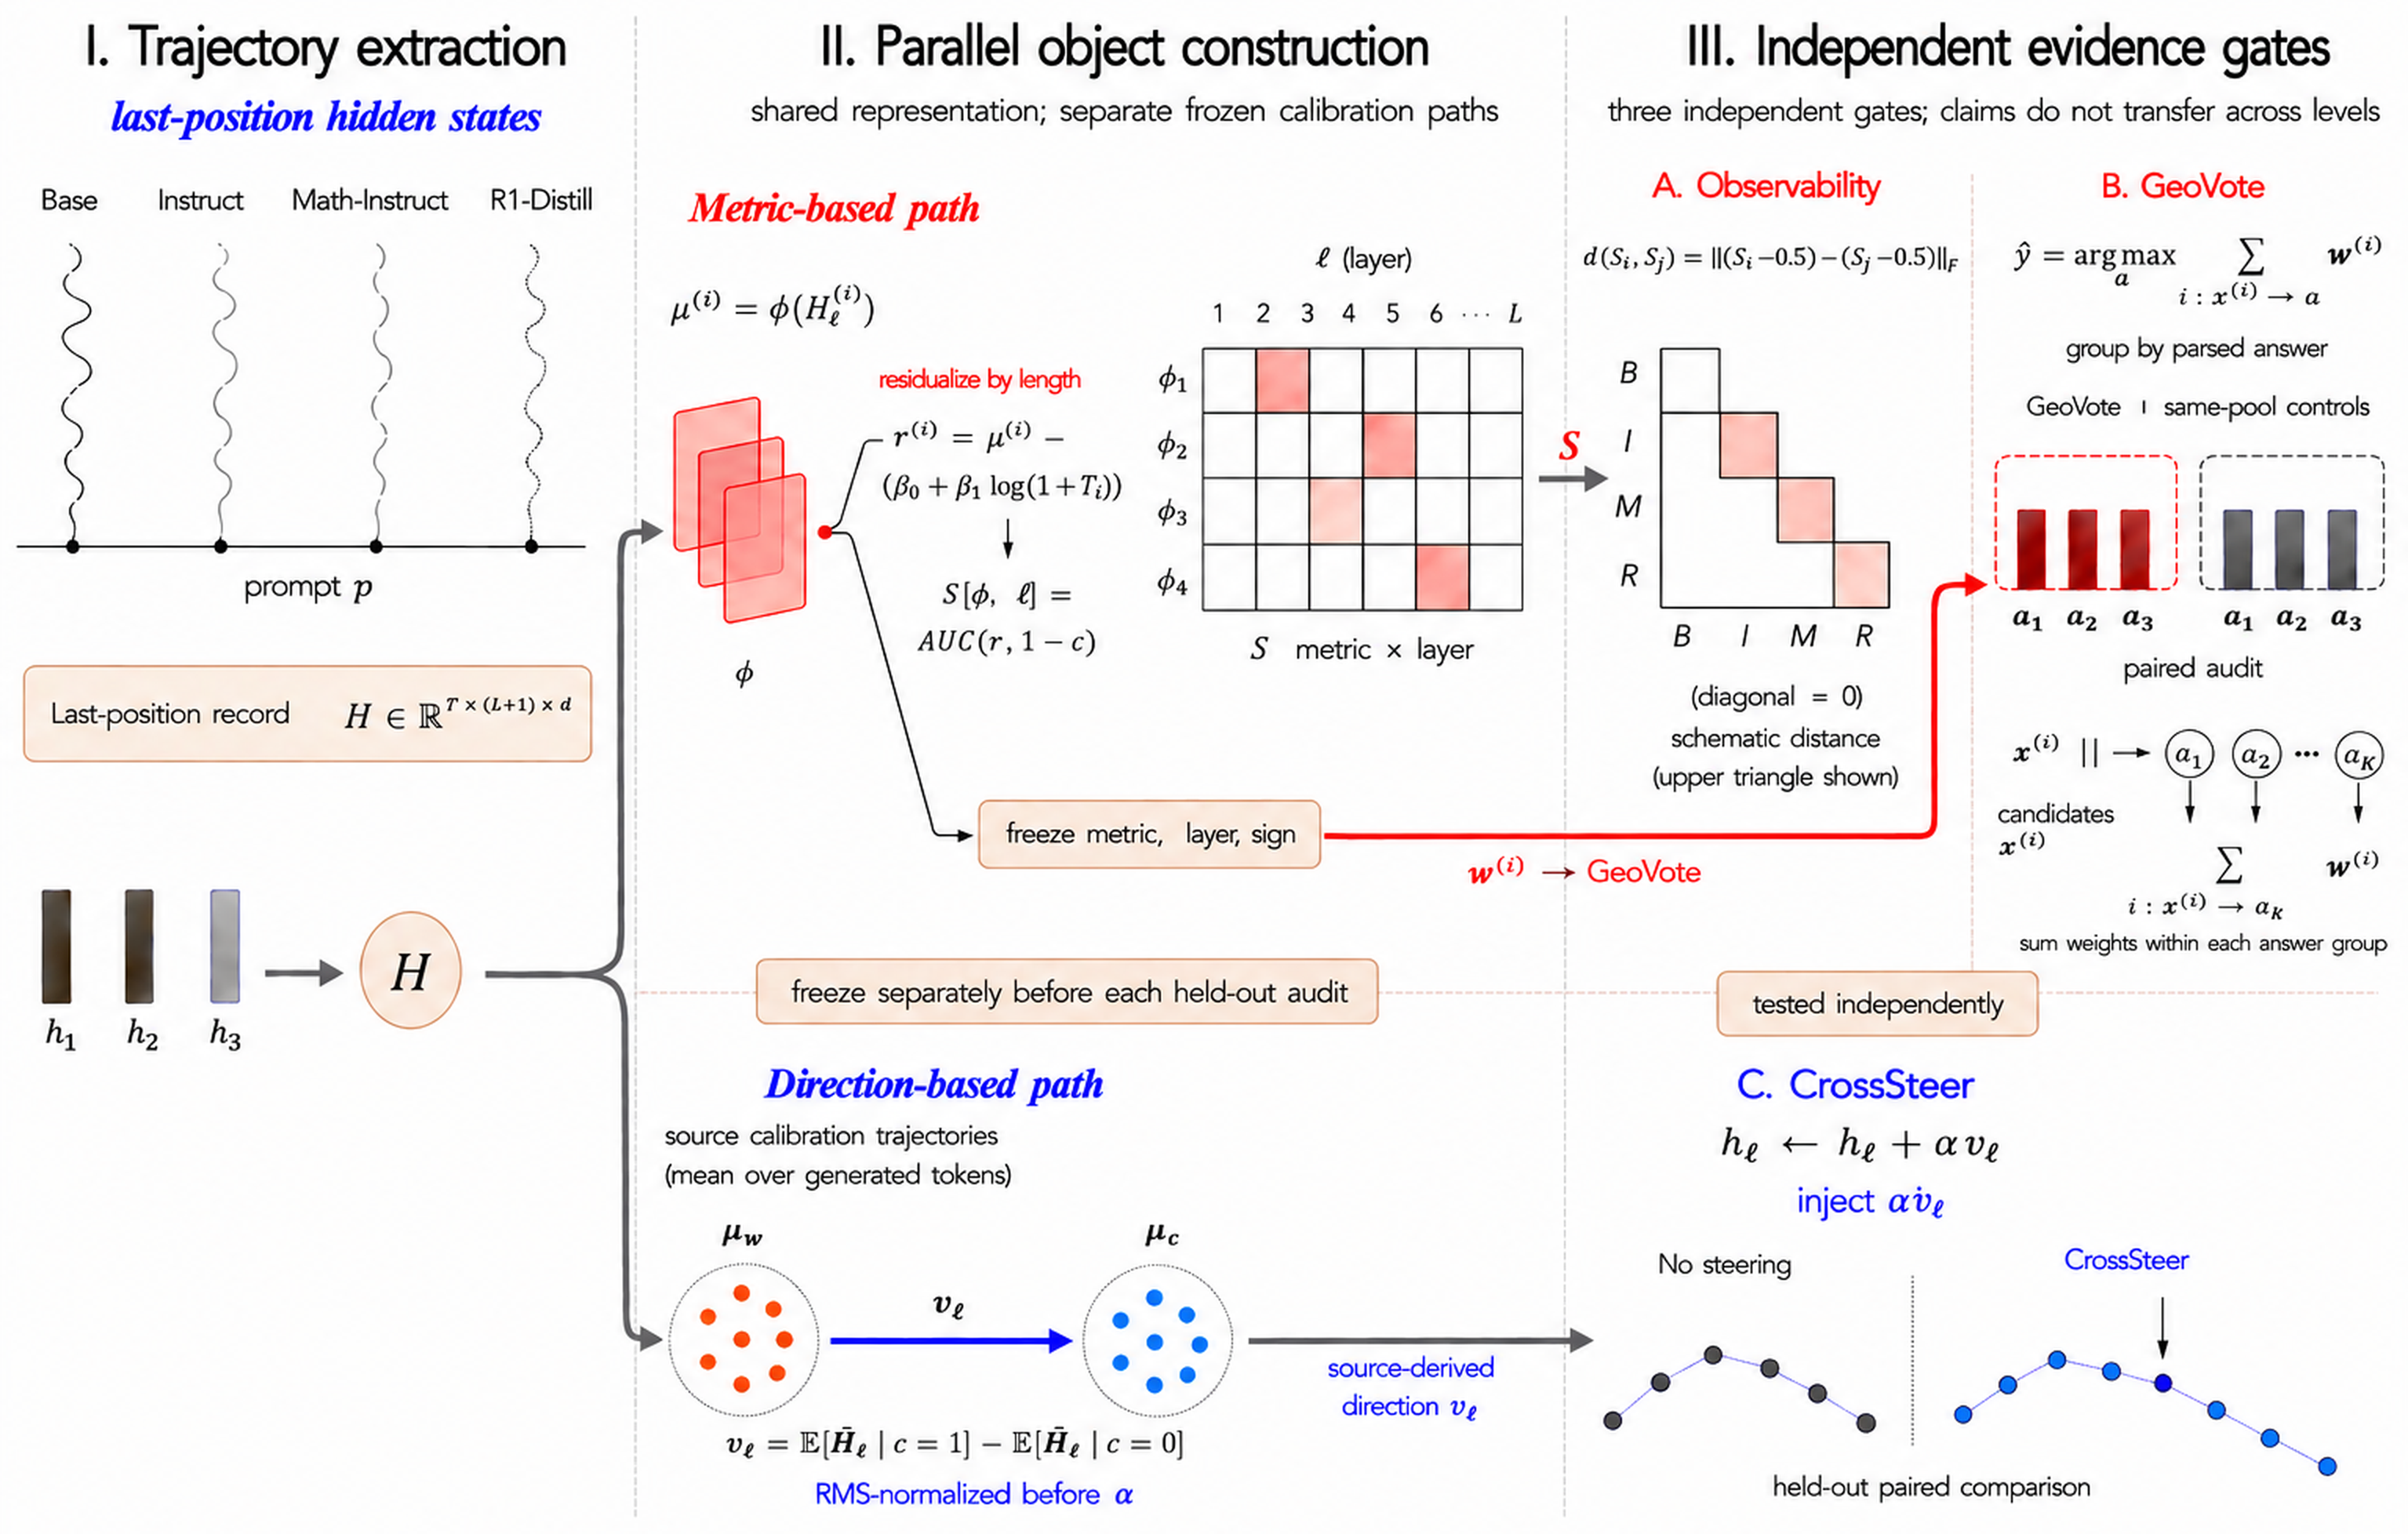
\includegraphics[width=0.88\linewidth]{figures/fig1_overview.png}
\caption{Conceptual overview of the controlled evaluation protocol. Matched
post-training variants share a last-position hidden-state record \(H\), from
which two frozen objects are built on separate calibration paths: a
metric--layer signature \(S\) (length-residualized AUC) and a source direction
\(v_\ell\) (token-mean class difference on \(H\), not on the residual \(r\)).
These objects are tested as three independent evidence gates---observability,
same-pool candidate selection (\textsc{GeoVote}; frozen \(\mu=\phi(H)\)), and
source-direction intervention (\textsc{CrossSteer})---with no cross-level
transfer of claims. Arrows show protocol flow, not a promised gain; matrices,
bars, and trajectories are schematic and do not encode measured results. Each
use is frozen before its own held-out audit.}
\label{fig:overview}
\end{figure*}

\paragraph{First question: is there a measurable association?}
We first use the signature as a diagnostic.  In the retained retrospective
artifacts for a controlled \textsc{Qwen2.5}-derived 1.5B family, the variants
share architecture, tokenizer, prompt, decoding rule, and diagnostic problem
slice.  They differ in
post-training, but they are not treated as a perfectly controlled causal chain.
We therefore ask the narrower question: do their metric--layer correctness
associations differ under the same extraction protocol?  We also audit whether
fine-grained nearest-neighbor relations change with scale and generation budget.
A separately preregistered fresh confirmation chain did not pass its truncation
eligibility gate, so the diagnostic claim remains retrospective and descriptive
(Section~\ref{sec:phenomenon}).

\paragraph{Second question: does the association help at inference time?}
We evaluate two possible uses of a frozen trajectory signal.
\textsc{GeoVote} (geometric voting) inserts a trajectory score into an existing
best-of-$N$ selector.  It is compared with majority voting, output-length
controls, length-residualized scores, and log probability.  \textsc{CrossSteer}
(cross-model steering) constructs a correct-minus-incorrect direction from
calibration trajectories and injects it at a target layer.  We compare source
transfer with target calibration, CAA, ActAdd, SAE activation,
coordinate-sparse, sign-reversed, matched-norm random, and no-steering controls.
All choices are separated into calibration, validation, and locked-test splits.

We distinguish three evidence levels.  An association asks whether geometry
separates correct from incorrect trajectories.  A selection result asks whether
that signal improves a final choice among the same candidates.  An intervention
result asks whether a frozen direction improves a locked target comparison.
A visible geometric difference does not automatically pass the latter two tests;
our claims therefore follow the paired, locked comparisons.

\paragraph{Contributions.}
\begin{itemize}[topsep=2pt,itemsep=2pt,leftmargin=*]
\item We introduce a reproducible protocol that represents each checkpoint by
a metric--layer matrix of length-residualized trajectory--correctness
associations.
\item Retained retrospective artifacts from a matched
\textsc{Qwen2.5}-derived family show different signature matrices under the
fixed protocol.  Bootstrap, budget, and scale audits delimit which descriptive
contrasts recur; a separately preregistered fresh confirmation chain did not
pass its truncation eligibility gate, so no universal or confirmatory
taxonomy claim is made.
\item We introduce and apply a three-level evidence standard that separates
observability from candidate-selection utility and intervention efficacy.
Same-pool controls show that \textsc{GeoVote} adds no reliable selection gain,
and a locked eight-method comparison finds no reliable source-transfer gain.  A
predeclared target-local five-label cell yields $+11$~pp after Holm correction ($p{=}0.0443$);
the complete non-monotone curve bounds the scope of that result.
\end{itemize}
